\documentclass[11pt]{article}

\usepackage[margin=1in]{geometry}
\usepackage{amsmath,amssymb,amsfonts}
\usepackage{braket}
\usepackage{graphicx}
\usepackage{microtype}
\usepackage{enumitem}
\usepackage[hidelinks]{hyperref}

\setlength{\parindent}{0pt}
\setlength{\parskip}{0.55em}

\title{\textbf{PHYS 3316 -- Quantum Physics I}\\
Class Notes -- 24 September 2026\\[0.4em]
\large Quantum Formalism -- ``Chopping Things Up'' (Ch.~3)}
\author{Eric R. Bittner}
\date{}

\begin{document}
\maketitle

\section{Vectors in Hilbert Space}

A state in quantum mechanics, $\ket{\psi}$, is a vector in a linear vector
space. Operators are linear transformations in the state space.

As an example, suppose we have a two-state system (qubit), with basis states
\[
\ket{\psi_0}
=
\begin{pmatrix}
1\\
0
\end{pmatrix},
\qquad
\ket{\psi_1}
=
\begin{pmatrix}
0\\
1
\end{pmatrix}.
\]

Let us write the Hamiltonian in this basis. Its matrix elements are
\[
H_{00}=\bra{\psi_0}H\ket{\psi_0}=\epsilon_0,
\]
\[
H_{10}=H_{01}^*
=
\bra{\psi_1}H\ket{\psi_0}
=
g,
\]
where $g$ may in general be complex, and
\[
H_{11}=\epsilon_1.
\]
Thus
\[
H=
\begin{pmatrix}
\epsilon_0 & g^*\\
g & \epsilon_1
\end{pmatrix}.
\]

We can define operators in the $\{\ket{\psi_0},\ket{\psi_1}\}$ basis. For
example,
\[
\sigma_x
=
\ket{\psi_1}\bra{\psi_0}
+
\ket{\psi_0}\bra{\psi_1},
\]
\[
\sigma_y
=
i\left(
\ket{\psi_1}\bra{\psi_0}
-
\ket{\psi_0}\bra{\psi_1}
\right),
\]
\[
\sigma_z
=
\ket{\psi_0}\bra{\psi_0}
-
\ket{\psi_1}\bra{\psi_1},
\]
and
\[
\sigma_0
=
\ket{\psi_0}\bra{\psi_0}
+
\ket{\psi_1}\bra{\psi_1}.
\]
These operators will become more familiar when we discuss spin-$1/2$ systems.

\section{Two-State Hamiltonian and Basis Rotation}

We can write the two-state Hamiltonian in the Pauli basis as
\[
H
=
a_0\sigma_0
+
a_x\sigma_x
+
a_y\sigma_y
+
a_z\sigma_z.
\]
Defining
\[
\Delta=\epsilon_0-\epsilon_1,
\]
the coefficients may be chosen as
\[
a_0=\frac{\epsilon_0+\epsilon_1}{2},
\qquad
a_x=\operatorname{Re}g,
\qquad
a_y=\operatorname{Im}g,
\qquad
a_z=\frac{\Delta}{2}.
\]
% Editorial note: the a_i subscripts on the blackboard are permuted relative
% to the written Pauli ordering; the physically equivalent coefficients above
% are consistent with the subsequent line H=(Delta/2)sigma_z+g sigma_x.

We now define a transformation that brings $H$ into diagonal form. Without
loss of generality, take $g$ to be real and drop the common energy shift,
so that
\[
H
=
\frac{\Delta}{2}\sigma_z
+
g\sigma_x.
\]

Define the rotation matrix
\[
T(\theta)
=
\begin{pmatrix}
\cos\theta & \sin\theta\\
-\sin\theta & \cos\theta
\end{pmatrix},
\qquad
T^\dagger T=1.
\]
We take
\[
\widetilde H=T^\dagger H T
\]
and define the rotated basis states by
\[
\ket{\psi_+}=T^\dagger\ket{\psi_0},
\qquad
\ket{\psi_-}=T^\dagger\ket{\psi_1}.
\]

Direct multiplication gives
\[
\widetilde H
=
\begin{pmatrix}
\frac{\Delta}{2}\cos(2\theta)-g\sin(2\theta)
&
g\cos(2\theta)+\Delta\cos\theta\sin\theta
\\[0.5em]
g\cos(2\theta)+\Delta\cos\theta\sin\theta
&
-\frac{\Delta}{2}\cos(2\theta)+g\sin(2\theta)
\end{pmatrix}.
\]

Choose $\theta$ so that the off-diagonal element vanishes:
\[
g\cos(2\theta)
+
\Delta\cos\theta\sin\theta
=
0.
\]
Using
\[
\sin(2\theta)=2\sin\theta\cos\theta,
\]
this becomes
\[
g\cos(2\theta)
+
\frac{\Delta}{2}\sin(2\theta)
=
0,
\]
or
\[
\boxed{
\cot(2\theta)
=
-\frac{\Delta}{2g}
}.
\]
Equivalently,
\[
\tan(2\theta)=-\frac{2g}{\Delta}.
\]

This is simply a rotation to a new basis within the same Hilbert space.

The diagonal elements are
\[
\widetilde E_+
=
\frac{\Delta}{2}\cos(2\theta)
-
g\sin(2\theta),
\]
\[
\widetilde E_-
=
-\frac{\Delta}{2}\cos(2\theta)
+
g\sin(2\theta).
\]
Using the diagonalization condition,
\[
\boxed{
E_\pm
=
\pm\frac{1}{2}\sqrt{\Delta^2+4g^2}
}.
\]

\section{Time Evolution and Coherent Oscillations}

Suppose we prepare the initial state in $\ket{\psi_0}$ and allow it to evolve
according to the Schr\"odinger equation. In the rotated basis,
\[
\ket{\psi_0}
=
\cos\theta\,\ket{\psi_+}
+
\sin\theta\,\ket{\psi_-}.
\]

Therefore
\[
\ket{\psi(t)}
=
e^{-iHt/\hbar}\ket{\psi_0}
=
\cos\theta\,
e^{-iE_+t/\hbar}\ket{\psi_+}
+
\sin\theta\,
e^{-iE_-t/\hbar}\ket{\psi_-}.
\]

To make the calculation easier, consider the resonant case
\[
\Delta=0.
\]
Then
\[
\cos\theta=\sin\theta=\frac{1}{\sqrt{2}},
\qquad
\theta=\frac{\pi}{4},
\]
and
\[
E_\pm=\pm g.
\]
Thus
\[
\ket{\psi(t)}
=
\frac{1}{\sqrt{2}}
\left[
e^{-igt/\hbar}\ket{\psi_+}
+
e^{+igt/\hbar}\ket{\psi_-}
\right].
\]

What is the probability that the system remains in $\ket{\psi_0}$ at time
$t$? We compute
\[
P_0(t)
=
\left|
\braket{\psi_0|\psi(t)}
\right|^2.
\]
Since
\[
\bra{\psi_0}
=
\frac{1}{\sqrt{2}}
\left(
\bra{\psi_+}
+
\bra{\psi_-}
\right),
\]
we obtain
\[
\braket{\psi_0|\psi(t)}
=
\frac{1}{2}
\left(
e^{-igt/\hbar}
+
e^{+igt/\hbar}
\right)
=
\cos\left(\frac{gt}{\hbar}\right),
\]
and therefore
\[
\boxed{
P_0(t)
=
\cos^2\left(\frac{gt}{\hbar}\right)
}.
\]

Writing
\[
\Omega=\frac{g}{\hbar},
\]
the system undergoes coherent oscillation between the states
$\ket{\psi_0}$ and $\ket{\psi_1}$. Since
\[
P_0(t)+P_1(t)=1,
\]
we have
\[
P_1(t)
=
\sin^2\left(\frac{gt}{\hbar}\right).
\]

\begin{figure}[ht]
\centering
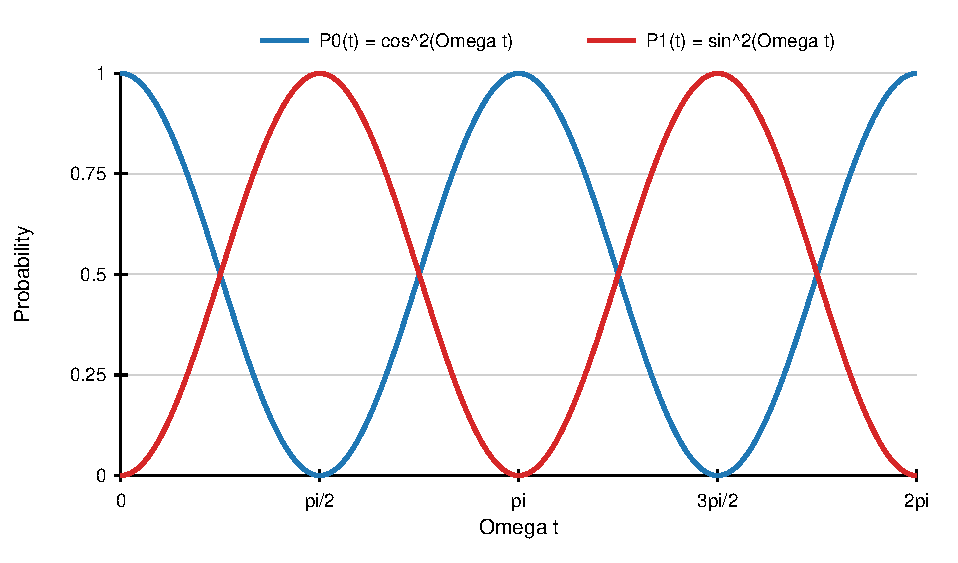
\includegraphics[width=0.72\textwidth]{figures/rabi_oscillations.pdf}
\caption{Coherent oscillation between the two basis states for $\Delta=0$.
Here $\Omega=g/\hbar$.}
\label{fig:rabi}
\end{figure}

\section{Some Operator Properties and Identities}

For operators $\widehat Q$ and $\widehat R$,
\[
(\widehat Q+\widehat R)\ket{\psi}
=
\widehat Q\ket{\psi}
+
\widehat R\ket{\psi}.
\]

For a product of operators,
\[
\widehat Q\widehat R\ket{\psi}
=
\widehat Q\left(\widehat R\ket{\psi}\right)
=
\widehat Q\ket{\psi'},
\]
where
\[
\ket{\psi'}=\widehat R\ket{\psi}.
\]

In general,
\[
\widehat Q\widehat R\ket{\psi}
\neq
\widehat R\widehat Q\ket{\psi}
\]
if
\[
[\widehat Q,\widehat R]\neq0.
\]

Functions of operators may be defined by power-series expansions. For example,
\[
e^{\widehat Q}
=
1+\widehat Q+\frac{1}{2!}\widehat Q^2
+\frac{1}{3!}\widehat Q^3+\cdots,
\]
\[
\frac{1}{1-\widehat Q}
=
1+\widehat Q+\widehat Q^2+\widehat Q^3+\cdots,
\]
and
\[
\ln(1+\widehat Q)
=
\widehat Q
-\frac{1}{2}\widehat Q^2
+\frac{1}{3}\widehat Q^3
-\frac{1}{4}\widehat Q^4
+\cdots.
\]

\paragraph{Homework.}
Prove these power-series identities.

Be careful with exponentials of noncommuting operators. In general,
\[
e^{A+B}\neq e^Ae^B
\]
when
\[
[A,B]\neq0.
\]

Suppose instead that we write
\[
e^{A+B}
=
e^Ae^Be^C.
\]
The Baker--Campbell--Hausdorff expansion begins as
\[
\ln(e^Ae^B)
=
A+B+\frac{1}{2}[A,B]+\cdots.
\]
Thus the compensating exponent begins with
\[
C
=
-\frac{1}{2}[A,B]+\cdots,
\]
so that
\[
e^{A+B}
=
e^Ae^B
e^{-\frac12[A,B]+\cdots}.
\]

In the special case
\[
[A,[A,B]]
=
[B,[A,B]]
=
0,
\]
the series terminates at this order.

\section{Unitary Transformations}

Quantum operators are often transformed by a unitary operator
\[
U=e^S,
\]
where $S$ is anti-Hermitian:
\[
S^\dagger=-S.
\]
Then
\[
U^\dagger=e^{-S}.
\]

A transformed operator may be written as
\[
\widetilde A
=
U^\dagger A U
=
e^{-S}Ae^S.
\]
Expanding in nested commutators gives
\[
\widetilde A
=
A
+
[A,S]
+
\frac{1}{2!}[[A,S],S]
+
\frac{1}{3!}[[[A,S],S],S]
+\cdots.
\]

Now suppose
\[
H=H_0+W,
\]
where $H_0$ is diagonal and $W$ is off-diagonal. In the $H_0$ basis,
\[
\bra{m}W\ket{n}\neq0
\quad (m\neq n),
\qquad
\bra{m}W\ket{m}=0.
\]

The transformed Hamiltonian is
\begin{align*}
\widetilde H
={}&
H_0
+
[H_0,S]
+
\frac{1}{2!}[[H_0,S],S]
+\cdots
\\
&+
W
+
[W,S]
+
\frac{1}{2!}[[W,S],S]
+\cdots.
\end{align*}

We choose $S$ so that $\widetilde H$ becomes more nearly diagonal. The simplest
choice is
\[
\boxed{
[H_0,S]=-W
}.
\]
With this condition,
\[
\widetilde H
=
H_0
+
\left(
\frac{1}{1!}-\frac{1}{2!}
\right)[W,S]
+
\left(
\frac{1}{2!}-\frac{1}{3!}
\right)[[W,S],S]
+\cdots.
\]

Returning to the two-state problem,
\[
H_0
=
\frac{\Delta}{2}\sigma_z,
\qquad
W=g\sigma_x.
\]
We require
\[
[H_0,S]=-W,
\]
or
\[
\frac{\Delta}{2}
[\sigma_z,S]
=
-g\sigma_x.
\]

Using
\[
[\sigma_i,\sigma_j]
=
2i\epsilon_{ijk}\sigma_k,
\]
and in particular
\[
[\sigma_x,\sigma_y]=2i\sigma_z,
\qquad
[\sigma_y,\sigma_z]=2i\sigma_x,
\]
take
\[
S=a\sigma_y.
\]
Since
\[
[\sigma_z,\sigma_y]
=
-2i\sigma_x,
\]
we obtain
\[
\frac{\Delta}{2}
a(-2i\sigma_x)
=
-g\sigma_x,
\]
which gives
\[
\boxed{
a=-i\frac{g}{\Delta}
}.
\]
Therefore
\[
S
=
-i\frac{g}{\Delta}\sigma_y.
\]

The corresponding unitary transformation is a rotation about the $y$ axis:
\[
U
=
e^{-i(g/\Delta)\sigma_y},
\qquad
U^\dagger
=
e^{+i(g/\Delta)\sigma_y}.
\]



%%%%%%%%%%%%%%%%%%%%%%%%%%%%%%%%%%%%%%%%%%%%%%%%%%%%%%%%%%%%%%%%%%%%%%%%%%
\section{Continuous Unitary Transformations}

Rather than evaluating the similarity transformation directly, it is often
useful to introduce a continuous parameter,

\[
A(\lambda)
=
e^{-\lambda S}Ae^{\lambda S},
\qquad
0\le\lambda\le1,
\]

so that

\[
A(0)=A,
\qquad
A(1)=e^{-S}Ae^{S}.
\]

Differentiating with respect to $\lambda$ gives

\[
\frac{dA(\lambda)}{d\lambda}
=
e^{-\lambda S}[A,S]e^{\lambda S}
=
[A(\lambda),S].
\]

For the two-level Hamiltonian we found

\[
S=-i\alpha\sigma_y,
\qquad
\alpha=\frac{g}{\Delta}.
\]

Define

\[
\sigma_z(\lambda)
=
e^{-\lambda S}\sigma_z e^{\lambda S},
\qquad
\sigma_x(\lambda)
=
e^{-\lambda S}\sigma_x e^{\lambda S}.
\]

Using

\[
[\sigma_z,\sigma_y]=-2i\sigma_x,
\qquad
[\sigma_x,\sigma_y]=2i\sigma_z,
\]

the equations of motion become

\[
\frac{d\sigma_z}{d\lambda}
=
-2\alpha\,\sigma_x,
\]

\[
\frac{d\sigma_x}{d\lambda}
=
2\alpha\,\sigma_z.
\]

Differentiating once more,

\[
\frac{d^2\sigma_z}{d\lambda^2}
=
-4\alpha^2\sigma_z,
\]

with initial conditions

\[
\sigma_z(0)=\sigma_z,
\qquad
\left.\frac{d\sigma_z}{d\lambda}\right|_{\lambda=0}
=
-2\alpha\sigma_x.
\]

The solution is

\[
\sigma_z(\lambda)
=
\sigma_z\cos(2\alpha\lambda)
-
\sigma_x\sin(2\alpha\lambda),
\]

and similarly

\[
\sigma_x(\lambda)
=
\sigma_x\cos(2\alpha\lambda)
+
\sigma_z\sin(2\alpha\lambda).
\]

Setting $\lambda=1$,

\[
e^{-S}\sigma_z e^S
=
\sigma_z\cos(2\alpha)
-
\sigma_x\sin(2\alpha).
\]

Expanding for small $\alpha$,

\[
\sigma_z(\lambda)
=
\sigma_z
-
2\alpha\lambda\,\sigma_x
-
2\alpha^2\lambda^2\,\sigma_z
+\cdots,
\]

which reproduces the Baker--Campbell--Hausdorff expansion,

\[
e^{-\lambda S}\sigma_z e^{\lambda S}
=
\sigma_z
+
\lambda[\sigma_z,S]
+
\frac{\lambda^2}{2}
[[\sigma_z,S],S]
+\cdots.
\]

This provides an exact SU(2) realization of the BCH series: the nested
commutators sum to a finite rotation generated by the Pauli algebra.


\end{document}
